\section{The Evaluation Sub-system: NPUKernelBench}\label{NPUKernelBench}

\subsection{Benchmark Overview}

\begin{comment}

\begin{figure}[t]
    \centering
    \includegraphics[width=1\linewidth]{latex/pdfs/NPUKernelBench_Overview.pdf}
    \caption{The proposed NPUKernelBench framework begins with Instructions and Kernel Tasks, which are jointly fed into the LLM to generate a structured Chain of Thought (CoT) and the corresponding Host and Kernel Code. These codes are then compiled and evaluated for correctness and performance on NPU hardware.}
    \label{fig:NPUKernelBench_framework}
\end{figure}

\end{comment}

%As illustrated in Fig.~\ref{fig:NPUKernelBench_framework}, the framework provides a standardized environment that supports the entire workflow of kernel development, validation, and performance optimization. Functioning as the core instrument for measuring the quality of generated kernels, the system is anchored by two pivotal components: \textit{Task Definition} and \textit{Evaluation Metrics}. Specifically, it pre-defines hierarchical tasks in the \textbf{Kernel Task} module and simultaneously integrates a large language model (LLM) to automate \textbf{Code Generation}. By interpreting kernel specifications, the system generates CANN-compliant Ascend C code—including both host- and kernel-side components—which can be directly compiled and executed. This process seamlessly connects to the comprehensive Automated Evaluation Pipeline, where the framework sequentially performs compilation checks, evaluates correctness against reference outputs, and measures performance metrics, thus enabling end-to-end assessment of kernel functionality and efficiency.

Figure~\ref{fig:framework} includes an overview of \href{https://github.com/weich97/NPUKernelBench}{\textcolor{blue}{NPUKernelBench}}, an end-to-end evaluation framework for assessing the ability of large language models (LLMs) to generate correct and efficient NPU kernels. The framework spans the full evaluation lifecycle, from task specification and code generation to compilation, hardware execution, and quantitative measurement.

Given a structured kernel task and corresponding instructions, NPUKernelBench prompts the LLM to generate both a structured chain-of-thought (CoT) representation and executable host-side and kernel-side code. The generated code is then compiled and executed on the NPU hardware, where functional correctness and execution performance are automatically evaluated against reference implementations.

By grounding evaluation in actual hardware behavior and enforcing full compilation and execution, NPUKernelBench enables objective, reproducible, and fine-grained analysis of kernel generation quality.

\subsection{Kernel Task: Hierarchical and Categorical Design}

%There is a fundamental challenge arises when we using large language models (LLMs) for NPU kernel development: \textit{how can we objectively and comprehensively evaluate the model’s true capability in writing efficient and correct NPU kernels?} Treating all kernels equally would obscure crucial differences in algorithmic complexity and input adaptability. For instance, an AI model capable of generating code for an element-wise addition may fail to handle the more intricate logic of an attention mechanism, or a model that excels at optimizing kernels for fixed input sizes may struggle with dynamic shapes such as variable batch sizes.

Evaluating LLMs for NPU kernel generation requires disentangling multiple sources of difficulty. Treating all kernels as a homogeneous benchmark obscures key variations in computational structure and interface requirements, leading to incomplete assessments of model capability.

NPUKernelBench addresses this challenge through a structured task design that decomposes kernel difficulty along two orthogonal dimensions: \emph{algorithmic complexity} and \emph{interface complexity}. Together, these dimensions form a hierarchical and categorical evaluation scheme that enables systematic analysis of both specialization and generalization behavior.

\begin{comment}

\textbf{(1) Core Algorithmic Complexity -- Defining Kernel Levels.}  
To evaluate a model’s ability to understand and implement algorithms of varying complexity, Table \ref{tab:kernels} categorize kernels into three levels:
\textbf{Level 1 (Simple Operators)} include basic element-wise or arithmetic operations, such as Add, Sub, and Equal, which involve linear data flow with minimal dependencies and almost no input-driven control logic, primarily testing a model’s capability to generate correct and efficient basic kernels;  
\textbf{Level 2 (Standard Operators)} focus on structured neural network operations, including Gelu,  MulSigmoid, and RmsNorm, which require handling local data dependencies, attribute-driven adjustments (e.g., stride, padding), and limited conditional branching, thus evaluating a model’s ability to implement common but moderately complex kernels with correct behavior;  
\textbf{Level 3 (Complex Operators)} comprise advanced kernels with dynamic or global dependencies, iterative computation, or input-driven control flow, such as Gemm, TopK, and parts of custom \texttt{Attention} cores, which demand careful handling of parallel execution, dynamic memory access, and complex logic, thereby assessing the model’s capacity for generating highly optimized and robust complex kernels.
\input{latex/tables/kernel_num}
\textbf{(2) Interface Complexity -- Static vs. Dynamic Shapes.} 
Our benchmark considers two kernel scenarios: \textit{static-shape} and \textit{dynamic-shape}. \textbf{Static-shape kernels} assume all tensor dimensions are known and fixed at compile time, allowing evaluation of whether a model can generate highly specialized kernels with optimal data transfer and computation scheduling. Even in this ideal setting, challenges remain in designing fine-grained tiling strategies, maximizing on-chip memory utilization, and ensuring efficient pipelining across computation stages.
In contrast, \textbf{dynamic-shape kernels} permit certain dimensions (e.g., batch size or sequence length) to be determined at runtime, assessing the model’s ability to generalize and adapt to varying input sizes. This scenario reflects real-world deployment conditions that demand flexibility and robustness. However, achieving such adaptability requires the model to handle dynamic dimensions, perform runtime memory computations, adjust loop boundaries and tiling strategies, and implement a robust host-side \texttt{InferShape} function.

\end{comment}

\paragraph{Algorithmic Complexity.}
Kernel tasks are categorized into three levels according to their inherent computational structure (Table~\ref{tab:kernels}). Level~1 tasks consist of simple element-wise or arithmetic operations with linear data flow. Level~2 tasks correspond to common neural network operators with structured computation and local dependencies. Level~3 tasks include operators with global dependencies, iterative computation, or dynamic control flow, such as \texttt{Gemm}, \texttt{TopK}, and attention-related kernels. These tasks place increasing demands on parallel reasoning, memory hierarchy management, and control logic synthesis.
\begin{table*}[ht]
\centering
\caption{Categorization of kernel tasks in NPUKernelBench.}
\resizebox{1\linewidth}{!}{
\begin{tabular}{clllll}
\toprule
\textbf{Level} & \textbf{Static-shape} & \textbf{Dynamic-shape} & \textbf{Categories} & \textbf{Representative} & \textbf{Tasks} \\
\midrule
\multirow{5}{*}{Level 1} &\multirow{5}{5.5cm}{Can linear data flow be mapped to fixed-size loops with deterministic memory access?}&\multirow{5}{5.5cm}{Can element-wise logic remain correct under runtime-determined tensor shapes?} & Comparison & Add, Equal & 3 \\
&&&Condition & IsFinite, IsInf & 3 \\
&&&Index & GatherV3, ScatterList & 2 \\
&&&Math &AddCustom, Sqrt & 26 \\
&&&TensorCreation &Arange, Eye &3 \\ \hline
\multirow{9}{*}{Level 2} &\multirow{9}{5.5cm}{Can structured computation exploit fixed tiling and local data reuse?}& \multirow{9}{5.5cm}{Can kernels generalize correctly across varying input sizes?} & Activation & Gelu, MulSigmoid & 14 \\
&&&Foreach & ForeachAbs, ForeachSqrt& 53\\
&&&Linalg & Cos, Matmul &2 \\
&&&Loss & CrossEntropyLoss, MseLoss & 4\\
&&&Mask & Tril, Triu & 3\\
&&&Norm & AddLayerNorm, RmsNorm &16\\
&&&Optim &ApplyAdamWV2& 2\\
&&&Reduce & MulSigmoidMulAddCustom & 4\\
&&&TensorMove & ExpandV2, ReverseSequence & 5\\ \hline
\multirow{4}{*}{Level 3} &\multirow{4}{6cm}{Can complex kernels with global dependencies and non-trivial execution logic be generated correctly?}& \multirow{4}{5.5cm}{Can kernels support dynamic shapes and control flow in complex execution scenarios?} & \multirow{2}{*}{GMM} & \multirow{2}{*}{Gemm, BasicMatmul} & \multirow{2}{*}{17} \\
&&& \multirow{2}{*}{Sort} & \multirow{2}{*}{TopKV3} & \multirow{2}{*}{1} \\
&&&&&\\
&&&&&\\
\midrule
&&&Total & 16 & 158 \\
\bottomrule
\end{tabular}}
\label{tab:kernels}
\end{table*}

\vspace{-1mm}
\begin{wrapfigure}{r}{0.48\linewidth}
    \centering
    \vspace{-10pt}
    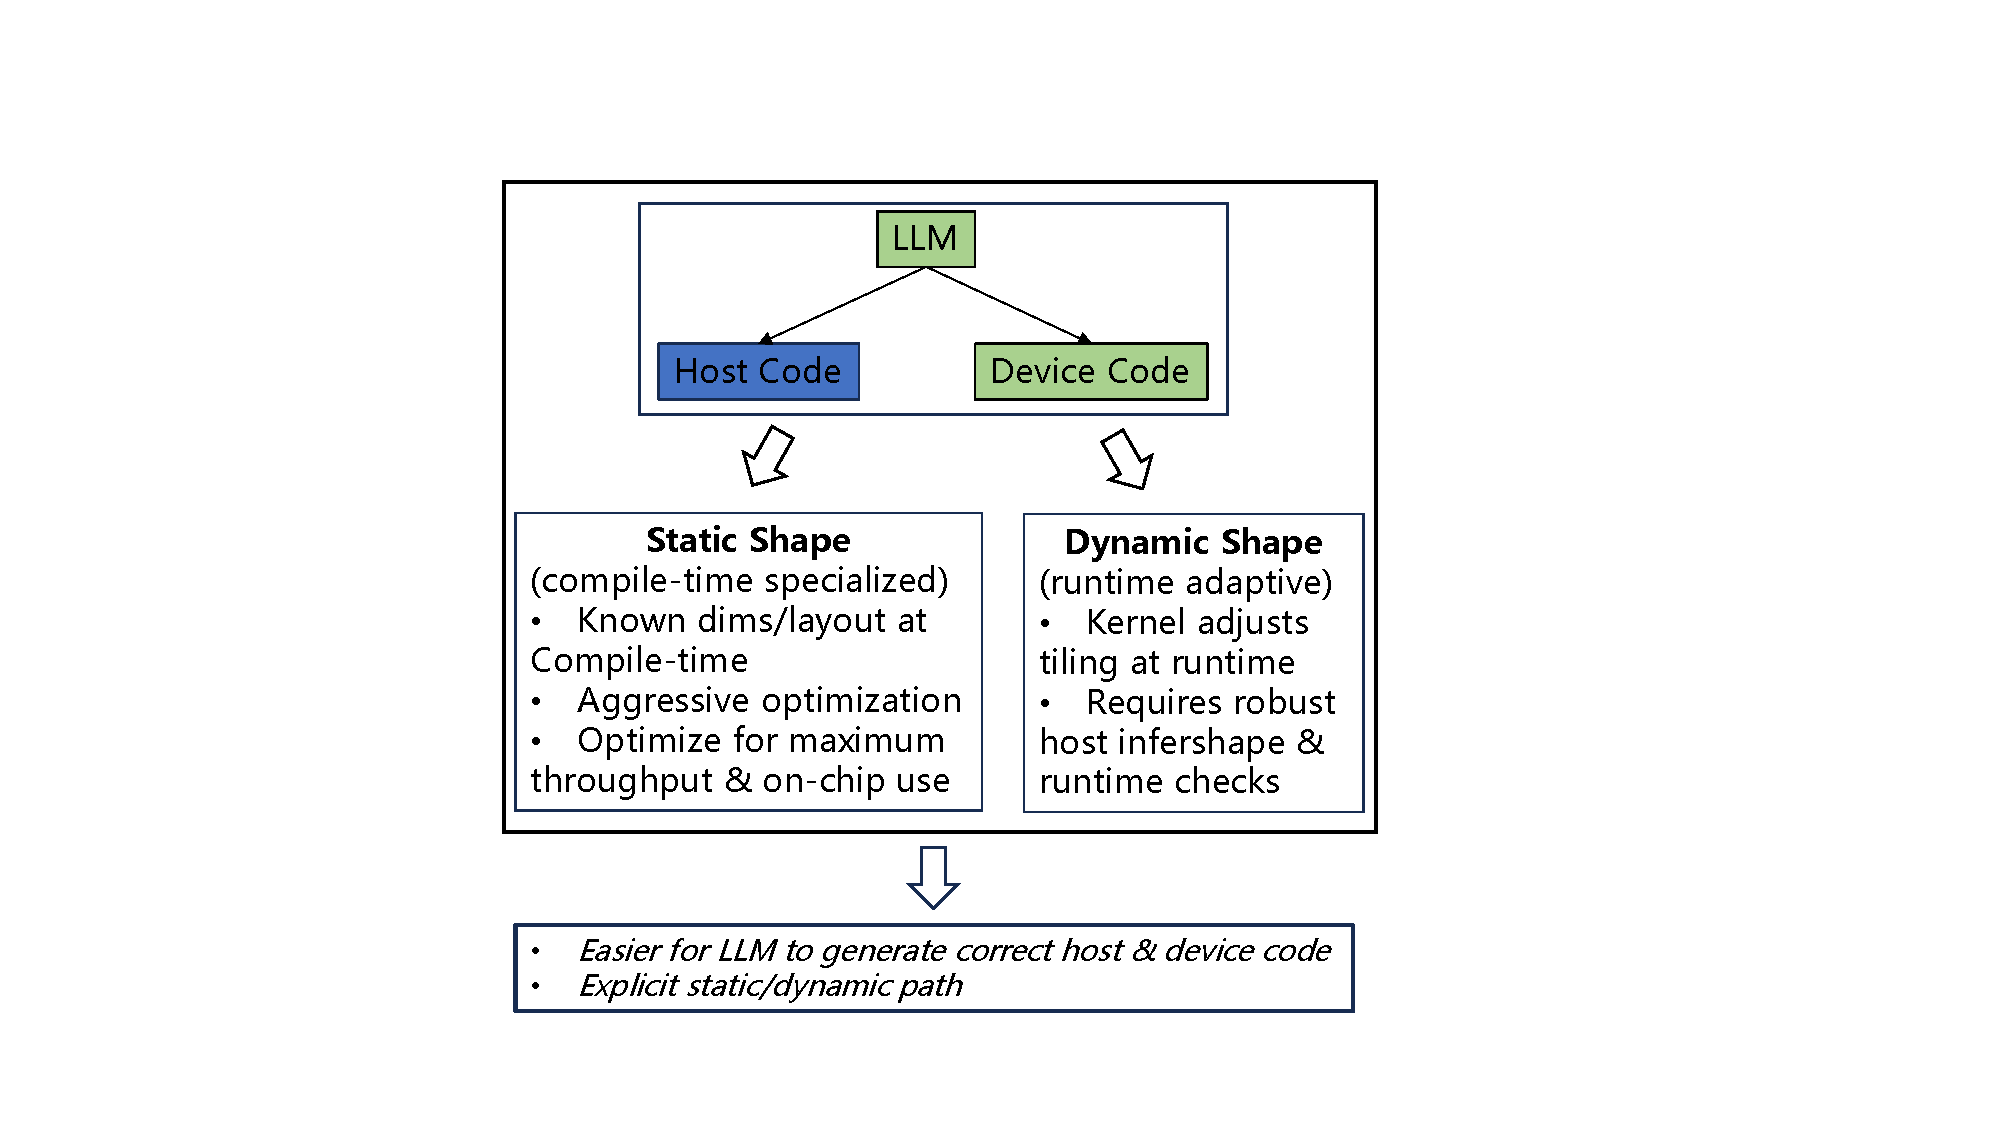
\includegraphics[
  width=\linewidth,
  trim=230pt 50pt 250pt 80pt,
  clip
]{pdfs/path.pdf}
    \vspace{-10pt}
    \caption{Dual-Path Evaluation Design.}
    \label{fig:dual_path}
    \vspace{-20pt}
\end{wrapfigure}
\paragraph{Interface Complexity.}
In addition to algorithmic difficulty, NPUKernelBench distinguishes between static-shape and dynamic-shape kernel tasks, shown in Figure~\ref{fig:dual_path}. Static-shape tasks assume compile-time known tensor dimensions and primarily evaluate specialization and optimization capability. Dynamic-shape tasks require kernels to adapt to runtime-determined dimensions, testing the model’s ability to generate robust host-side logic for shape inference, tiling computation, and control flow.




\subsection{Standardized Generation Interface}\label{sec_generate_kernel}
%The NPUKernelBench integrates a large language model (LLM) as a kernel generator to generate kernel code for the Ascend platform. Its workflow is structured around two key aspects: designing effective prompts to guide the LLM (\textit{Prompt Construction}) and specifying the precise content that the model should generate (\textit{What Content the Model Needs to Generate}). By combining carefully crafted prompts with clearly defined generation objectives, the module ensures that the LLM can understand operator requirements and produce well-structured code files.

To ensure fair and reproducible evaluation, NPUKernelBench defines a standardized generation interface that constrains both the input prompt and the structure of the generated code. This design bridges the gap between probabilistic LLM outputs and the deterministic requirements of the NPU compilation and execution pipeline.


%To ensure fair and reproducible evaluation, NPUKernelBench enforces a standardized generation interface that constrains both the input provided to the LLM and the structure of the generated output. This design bridges the gap between probabilistic text generation and the strict requirements of NPU compilation and execution.

\subsubsection{Prompt Formulation}
As illustrated in Tables~\ref{tab:prompt_ins} and \ref{tab:kernel_gen}, the prompt provided to the LLM integrates three complementary components: (1) task specification via API descriptions, (2) structural scaffolding through host and kernel code templates, and (3) role-based and formatting constraints. Together, these components provide sufficient semantic grounding and structural guidance for generating compilable Ascend C code.

%API description (\texttt{API\_Desc.md}) defines the kernel’s functionality and interface in a machine-readable markdown format. As show in Table~\ref{tab:kernel_gen}, it includes the mathematical formulation, computation process, input/output tensor specifications (names, data types, shapes, layouts, and attributes), and any constraints or hardware-specific notes. For instance, in the matrix multiplication example, the prompt explicitly describes the computational rule
%$C_{ij} = \sum_{p=1}^{k} A_{ip} B_{pj}$
%and details precision-handling strategies such as mixed-precision accumulation.
%\input{latex/tables/prompt_instructions}
%To ensure that the generated kernel code conforms to the expected software architecture and coding conventions, the framework provides pre-defined templates that serve as structural scaffolds for host and kernel implementations. These templates, located in the \texttt{tasks/.../question/} directory of each task within NPUKernelBench, specify the required code organization and interfaces. The host template defines kernel registration and tiling configuration, while the kernel template specifies the device computation entry point (e.g., \texttt{basic\_matmul\_kernel}). Table \ref{tab:kernel_gen} in Appendix show a whole template for generating Ascend kernel code.
%By leveraging these templates, the framework allows the LLM to focus on implementing computational logic rather than boilerplate, thereby enhancing generation consistency and reliability.
\textbf{Task Specification via API Description.} The core functional requirements are encapsulated in \texttt{API\_Desc.md}. As shown in Table~\ref{tab:kernel_gen}, this module translates the mathematical definition of the kernel into machine-readable specifications, detailing input/output tensor attributes (shapes, data types, layouts) and hardware constraints. For example, for a matrix multiplication kernel, the prompt explicitly formalizes the computation rule $C_{ij} = \sum_{p=1}^{k} A_{ip} B_{pj}$ and specifies precision modes, ensuring the model grounds its generation in accurate arithmetic logic.

\textbf{Structural Scaffolding via Code Templates.} To decouple algorithmic logic from boilerplate syntax, NPUKernelBench injects pre-defined code templates located in the \texttt{tasks/.../question/} directory. The prompt includes a host template (defining runtime registration and tiling interfaces) and a kernel template (specifying device-side entry points, e.g., \texttt{basic\_matmul\_kernel}). Table \ref{tab:kernel_gen} in the Appendix demonstrates a full template instance. This scaffolding forces the LLM to complete valid C++ structures rather than generating free-form text, significantly improving the compilability of the output.
\begin{wraptable}{l}{0.5\textwidth}
\vspace{-10pt}
\centering
\begin{tcolorbox}[
      sharp corners,
      colframe=reforange,
      colback=reforange!5,
      colbacktitle=reforange!15,
      coltitle=reforange,
      boxrule=0.4pt,
      title={\textbf{Instructions}},
      fonttitle=\bfseries\small,
      left=0.5pt,
      right=0.5pt,
      top=0.5pt,
      bottom=0.5pt
    ]
{\small
\begin{itemize}[leftmargin=*, itemsep=1pt, parsep=0pt, topsep=2pt]
    \item \textbf{Role:} "You are a professional Ascend kernel development engineer."
    \item \textbf{Target Language and API:} "Please use Ascend C for development."
    \item \textbf{Code Style Requirements:} "Ensure high code readability and include necessary comments."
    \item \textbf{Output Format Requirements:} "Generate separate Kernel and Host code: the Kernel defines <kernel\_name>\_kernel, and the Host declares Operator<OperatorName>Paras and implements the corresponding computation logic."
    \item \textbf{Key Information Reminder:} "Pay attention to handling the tensor data types, shapes, and layouts properly."
\end{itemize}
}
\end{tcolorbox}
\vspace{-10pt}
\captionof{table}{General instructions used in the prompt.}
\label{tab:prompt_ins}
\vspace{-10pt}
\end{wraptable}

At the beginning of a prompt, there are usually several general instructions, as illustrated in the left Table~\ref{tab:prompt_ins}. These instructions provide meta-level guidance that defines the model’s behavior, coding conventions, and output formatting. Specifically, they include explicit role prompts (e.g., adopting the perspective of a professional Ascend kernel engineer), target language and environment specifications (e.g., using Ascend C), code style requirements (e.g., ensuring readability and including necessary comments), and output format constraints (e.g., generating separate Kernel and Host code with clearly defined function and structure names). By providing sufficiently detailed instructions, the framework ensures that the LLM can follow consistent generation patterns and produce code that aligns with the target development standards.

\textbf{Role-Based Constraints.} The prompt begins with meta-instructions (Table~\ref{tab:prompt_ins}) that configure the model's persona (e.g., "Professional Ascend Kernel Development Engineer") and impose strict formatting rules. These instructions explicitly forbid conversational filler and mandate the separation of Host and Kernel code blocks. By formalizing these constraints, the framework ensures that the raw output from the LLM requires minimal post-processing before entering the compilation pipeline.

%Overall, the construction of a complete prompt follows a clear sequential process that integrates all necessary information for kernel generation. 
%First, the framework reads the task’s \texttt{api\_desc.md}, providing the model with a precise understanding of the kernel’s functionality and interface. 
%Next, the host and kernel code templates from the \texttt{question/} directory are incorporated, defining the expected structure and organization of the generated code. 
%Finally, general instructions specifying role, coding conventions, and output format are appended to guide the model’s behavior. 
%By integrating these elements in sequence, the framework ensures that the LLM receives all necessary information in a coherent and structured manner, enabling the generation of consistent and semantically correct kernel code.

Overall, the prompt formulation follows a deterministic sequence: ingesting the \texttt{api\_desc.md}, appending structural templates, and prepending constraint instructions. This creates a cohesive input context that maximizes the model's potential for generating compliant Ascend C code.

%On the input side, each prompt integrates three complementary components: (1) a formal API-based task specification, (2) structural code templates for host and kernel logic, and (3) explicit generation constraints that define coding conventions and output format. Together, these components provide sufficient context and structure while preventing unconstrained or ill-formed outputs.

\begin{comment}

The prompt provided to the LLM integrates three complementary components: (1) task specification via API descriptions, (2) structural scaffolding through host and kernel code templates, and (3) role-based and formatting constraints. Together, these components provide sufficient semantic grounding and structural guidance for generating compilable Ascend C code.

Task specifications are encoded in \texttt{API\_Desc.md}, which formalizes the mathematical definition of the kernel and specifies tensor attributes, precision modes, and hardware constraints. Structural scaffolding is provided through predefined host and kernel templates, which enforce valid C++ structure and isolate algorithmic logic from boilerplate syntax. Finally, role-based constraints define the model’s persona, coding conventions, and output format, ensuring consistency across generated samples.

\end{comment}

\subsubsection{Output Code Specification \& Dual-Path Evaluation}

NPUKernelBench enforces a strict output code specification to enable fully automated compilation and execution. Based on this specification, the framework supports a dual-path evaluation mechanism that assesses kernel generation capability under different system assumptions.

Specifically, NPUKernelBench supports two complementary evaluation paths. In the \emph{Device-Only Path}, the framework provides a fixed, pre-optimized host driver and evaluates the LLM solely on its ability to generate correct and efficient kernel-side code. This setting isolates the model’s fundamental capability in implementing core computational logic on the NPU and is particularly suitable for L1/L2 operators with minimal control flow. In contrast, the \emph{Host+Device Path} evaluates the model’s ability to generate complete, deployable operators. Under this setting, the LLM is required to produce both host-side control logic and kernel-side implementation, reflecting realistic deployment scenarios where runtime scheduling, shape inference, and dynamic memory management are essential.

\begin{comment}

In the \emph{Device-Only} path, a fixed host driver is provided and evaluation focuses exclusively on kernel-side code generation. In the \emph{Host+Device} path, the model is required to generate both host-side control logic and kernel-side implementation, reflecting realistic deployment scenarios involving shape inference, tiling computation, and runtime scheduling.

\end{comment}

%\textbf{a. Host-side code.}  This code runs on the CPU (host) and is responsible for preparing data, invoking the kernel, and processing results. The LLM is expected to:  
%\begin{itemize}
%    \item Define the parameter structure (\texttt{Operator<OperatorName>Paras}) for parsing and passing kernel attributes.  
%    \item Implement the \texttt{InferShape} function to derive output shapes from input tensors.  
%    \item Implement or invoke the Tiling function to compute kernel block information and parameters.  
%    \item Implement the logic for selecting kernel launch \texttt{BlockDim}.
%\end{itemize}

To support the Host+Device path, the output specification requires the generated code to instantiate three logically distinct but tightly coupled components within the provided templates (Table~\ref{tab:kernel_gen}). First, the host-side logic executes on the CPU and is responsible for orchestrating operator execution. This includes defining parameter structures for host–device communication, performing shape inference to derive output tensor dimensions at runtime, computing tiling parameters tailored to the target NPU architecture, and configuring kernel launch dimensions. Second, the kernel-side logic executes on the NPU AI Core and implements the parallel computation itself. The generated kernel must conform to the Ascend C programming model, correctly manage on-chip memory hierarchies, synchronize parallel execution, and employ SIMD-style computation with techniques such as double buffering to overlap data movement and computation. Finally, for operators with decoupled tiling logic, the framework expects an explicit tiling structure definition that bridges host-side tiling computation and kernel-side execution.

\begin{comment}

To support this comprehensive Host+Device path, the framework requires the LLM to instantiate three distinct logic components within the provided templates (Table~\ref{tab:kernel_gen}):

\textbf{a. Host-side Logic.} Executing on the CPU, this component manages the runtime environment. The framework requires the model to: \begin{itemize} \item Define the parameter structure (\texttt{Operator<Name>Paras}) for host-device communication. \item Implement \texttt{InferShape} logic to calculate output tensor dimensions dynamically. \item Compute Tiling parameters to optimize data block sizes for the specific NPU architecture. \item Configure the kernel launch dimensions (\texttt{BlockDim}). \end{itemize}

\textbf{b. Kernel-side Logic.} Executing on the NPU's AI Core, this component contains the parallel computational logic. The specification requires:  
\begin{itemize}
    \item Adherence to the Ascend C function signature (e.g., \texttt{extern ``C'' \_\_global\_\_ \_\_aicore\_\_ void <kernel\_name>(...)}).  
    \item Implementation of the Single Instruction Multiple Data (SIMD) logic, including double-buffering for data movement and vector/matrix computation instructions.
    \item Proper handling of synchronization barriers and memory hierarchies (Global Memory $\leftrightarrow$ Local Memory).
    \item Support different data types and shapes according to the specifications in \texttt{API\_Desc.md}.
\end{itemize}

\textbf{c. Tiling Structure Definition.}  
For complex operators requiring decoupled tiling logic, the framework expects a dedicated header definition that encapsulates the tiling data structure, ensuring it aligns with the host-side calculation.
% \begin{itemize}
%     \item Define the tiling structure or class used to organize and manage block-level computation parameters.
% \end{itemize}

\end{comment}

%In summary, we expect LLM to generate a complete Ascend operator C++ implementation—including Kernel, Host, and optionally Tiling logic, based on the semantic description in \texttt{API\_Desc.md} and the structural guidance of the code templates. The generating code must be functionally correct, syntactically compliant, and ready for compilation and execution within the framework. 
\begin{comment}

\vspace{1ex}
\noindent\textbf{Enabling Comprehensive Scenario Evaluation.}
The flexibility of this dual-path architecture and strict specification establishes NPUKernelBench as the first framework capable of comprehensively assessing kernels in two typical industrial scenarios:

\begin{enumerate}
    \item \textbf{Static Shape Optimization:} By analyzing the generated Kernel and Tiling logic, the framework evaluates the model's ability to produce extremely optimized code for fixed dimensions. Key assessment points include the design of tiling strategies, efficient management of on-chip memory (\texttt{LocalTensor}), and the optimization of computation/memory access pipelines.
    
    \item \textbf{Dynamic Shape Robustness:} Leveraging the \textbf{Host+Device Path}, the framework assesses the model's generalization ability. Since tensor shapes are unknown until runtime, the generated Host code must possess adaptive logic (e.g., dynamically calculating Tiling parameters and loop boundaries in \texttt{InferShape}). This effectively tests the robustness of the LLM-generated code in real-world, dynamic deployment environments.
\end{enumerate}

\end{comment}

This dual-path design enables NPUKernelBench to comprehensively evaluate kernel generation capability across two representative industrial scenarios, shown in Figure~\ref{fig:dual_path}. For \emph{static shape optimization}, the framework analyzes the generated kernel and tiling logic to assess whether the model can produce highly optimized code for fixed problem sizes, focusing on tiling strategy design, efficient use of on-chip memory, and compute–memory pipeline optimization. For \emph{dynamic shape robustness}, enabled by the Host+Device path, the framework evaluates the model’s ability to generalize to runtime-varying tensor shapes. In this setting, correctness and performance depend on adaptive host-side logic—such as dynamically computed tiling parameters and loop bounds—thereby testing the robustness of LLM-generated code in realistic deployment environments.


%On the output side, the framework requires the LLM to generate code that conforms to a fixed specification, enabling direct compilation and execution without manual intervention. Importantly, this specification supports two evaluation modes. In a \textit{device-only} mode, the LLM is evaluated on its ability to implement core kernel logic given a fixed host driver. In a \textit{host--device} mode, the model must generate a complete operator, including host-side control logic and kernel-side computation, reflecting realistic deployment scenarios.

By standardizing both prompt formulation and output structure, NPUKernelBench isolates model capability from prompt engineering artifacts and ensures that evaluation outcomes reflect genuine differences in kernel generation ability rather than formatting or interface inconsistencies.

\subsection{Automated Evaluation Pipeline}

NPUKernelBench is not merely a collection of test cases but a resilient, end-to-end automation framework designed to bridge the gap between model generation and rigorous hardware verification. As illustrated in Fig.~\ref{fig:framework}, the pipeline seamlessly integrates four traditionally isolated stages: \textit{Code Generation}, \textit{Compilation}, \textit{Correctness Verification}, and \textit{Performance Benchmarking}.

\begin{comment}

As illustrated in Fig.~\ref{fig:NPUKernelBench_framework}, NPUKernelBench implements a fully automated evaluation pipeline that integrates code generation, compilation, correctness verification, and performance benchmarking. The entire process is executed from a single entry point with unified configuration, enabling large-scale and reproducible evaluation.

To support high-throughput evaluation, the framework adopts a concurrent execution model with strict fault isolation. Each kernel is compiled and executed in an independent subprocess, preventing individual failures from disrupting the global pipeline. Timeout control, automatic retries, and resource cleanup further ensure robustness under long-running experiments.

\end{comment}

\subsubsection{End-to-End Architecture and Concurrency}
%To facilitate large-scale, reproducible experiments (e.g., $N=100$ samples per task), the framework adopts a "One-Click" design philosophy. Researchers can initiate the entire workflow through a single entry point (\texttt{run\_multi\_test.py}) configured via a unified definition file (\texttt{base\_config.yaml}), eliminating manual handovers between stages.

%To support the evaluation of thousands of samples across complex NPU operators, the pipeline incorporates a \textbf{Robust High-Concurrency Mechanism}:

To support large-scale and reproducible experiments (e.g., $N \geq 100$ samples per task), the framework follows a \emph{one-click} execution philosophy. The entire evaluation process is initiated from a single entry point (\texttt{run\_multi\_test.py}) and configured through a unified definition file (\texttt{base\_config.yaml}), eliminating manual intervention and reducing inconsistencies across experimental runs.

At scale, evaluating thousands of LLM-generated kernels across diverse NPU operators requires not only parallelism but also strong fault isolation. To this end, NPUKernelBench adopts a high-concurrency execution model based on Python \texttt{multiprocessing}, enabling parallel compilation and execution to maximize host CPU and NPU utilization. Each kernel evaluation is executed within a strictly isolated subprocess, ensuring that fatal errors—such as segmentation faults, illegal memory access, or NPU runtime exceptions—are contained locally and never propagate to disrupt the global pipeline.

Given the stochastic nature of LLM outputs and the complexity of hardware execution, the pipeline further incorporates native stability mechanisms to guarantee long-running robustness. Specifically, timeout control is used to proactively terminate non-terminating kernels or hardware hangs, while an automatic retry mechanism mitigates transient failures caused by network instability during API calls or temporary resource contention. In parallel, an active resource monitor enforces strict cleanup of host memory and NPU VRAM after each subprocess terminates, preventing resource leakage and ensuring consistent system behavior throughout extended batch evaluations.

Beyond execution robustness, NPUKernelBench is designed as a dedicated benchmarking suite with a structured, multi-level evaluation methodology tailored to custom NPU kernels. The framework evaluates generated operators along two primary dimensions: correctness and utilization, while adhering to three guiding principles. First, \emph{Correctness First} establishes functional validity as a prerequisite for any performance assessment. Second, \emph{Performance-Oriented Evaluation} emphasizes the effective utilization of NPU hardware resources once correctness is ensured. Third, \emph{Multi-Level Difficulty} introduces progressively more challenging tasks, enabling systematic assessment of optimization capability from basic implementations to highly tuned kernels.

These principles are realized through a fully automated evaluation pipeline comprising three tightly integrated stages: compilation evaluation, correctness evaluation, and performance evaluation. Generated kernels are first compiled to verify syntactic and build correctness, then executed on available NPU devices to validate numerical accuracy, and finally benchmarked to collect performance metrics such as execution latency and resource utilization. All stages are scheduled and executed in parallel whenever possible, with detailed logs and intermediate results recorded automatically. This design enables large-scale, objective, and reproducible evaluation of kernel generation quality with minimal human intervention.

\begin{comment}

\begin{itemize}
    \item \textbf{Parallelism \& Strict Isolation:} The framework leverages \texttt{multiprocessing} to parallelize compilation and execution, maximizing Host CPU and NPU utilization. Crucially, each evaluation task runs in a strictly isolated subprocess. This sandbox design ensures that a single kernel failure (e.g., a segmentation fault or NPU memory overflow) never propagates to crash the main pipeline.
    
    \item \textbf{Stability Assurance:} To handle the stochastic nature of LLMs and hardware interactions, the pipeline includes native \textbf{Timeout Handling} and \textbf{Auto-Retry} mechanisms. Transient failures caused by network fluctuations (during API calls) or resource contention trigger automatic retries, while infinite loops or hardware hangs are preemptively terminated to maintain overall progress.
    
    \item \textbf{Resource Recycling:} An active monitor tracks system resources, enforcing strict garbage collection of CPU memory and NPU VRAM after each subprocess terminates. This prevents resource leakage during long-running batch evaluations, ensuring consistent performance from the first sample to the last.
\end{itemize}

To comprehensively evaluate the capabilities of custom kernels on NPU, \textit{NPUKernelBench} is designed as a dedicated benchmarking suite featuring a structured and multi-level evaluation framework. Specifically, it assesses kernel implementations across two key dimensions, \textbf{correctness} and \textbf{efficiency}, while adhering to three core principles that ensure both scientific rigor and practical usability on the Ascend platform. Among them, \textit{Correctness First} underscores that functional accuracy serves as the foundation of all evaluations, \textit{Performance Goal} encourages developers to pursue maximal hardware efficiency once correctness is guaranteed, and \textit{Multi-level Difficulty} introduces progressively challenging tasks to assess optimization capability from basic to advanced levels.

Building on these principles, \textit{NPUKernelBench} employs a highly automated evaluation pipeline that ensures objectivity and reproducibility. The pipeline includes three stages: \textbf{compilation evaluation}, \textbf{correctness evaluation}, and \textbf{performance evaluation}. Each stage is executed in parallel whenever possible to improve efficiency. Generated kernels are compiled to check build correctness, tested for functional accuracy across available NPU, and subsequently benchmarked for performance metrics such as execution time and resource utilization. Throughout the process, the framework automatically manages task scheduling, logs detailed progress, and stores intermediate results, enabling large-scale, consistent, and transparent evaluation with minimal human intervention.

\end{comment}

\subsubsection{Compilation Evaluation}
In this stage, each generated kernel in Sec.~\ref{sec_generate_kernel} is first verified to ensure that it conforms to the Ascend C syntax and can be successfully compiled. To achieve this, the kernel is processed using the Ascend C compiler, and the compilation status is recorded as either success or failure. Meanwhile, detailed logs are stored in the \texttt{log/} directory of each kernel sample, which allows developers to inspect the corresponding \texttt{log\_file} in order to identify and diagnose any compilation errors. To illustrate this process, Table~\ref{tab:comp_log} presents a sample compilation log, highlighting the successful build of the \texttt{Sqrt} kernel from Level 1.

\begin{table}[H]
\vspace{-10pt}
\centering
\begin{tcolorbox}[
      sharp corners,
      colframe=refpurple,
      colback=refpurple!5,
      colbacktitle=refpurple!15,
      coltitle=refpurple,
      boxrule=0.4pt,
      title={\textbf{Compilation Log}},
      fonttitle=\bfseries\small,
      left=0.5pt,
      right=0.5pt,
      top=0.5pt,
      bottom=0.5pt
    ]
    \begin{lstlisting}[style=mystyle]
[INFO] Task lvl1_categoryMath_Sqrt_sample0 compile result:
==========================================================================================================
CompileResult:
success = True
log_file:
runs/msopgen/lvl1/Math/Sqrt/fixed_case_0/sample0/log/lvl1_categoryMath_Sqrt_sample0_compile.log
==========================================================================================================
\end{lstlisting}
\end{tcolorbox}
\captionof{table}{Compilation log of the \texttt{Sqrt} kernel using the Ascend C compiler. }
\label{tab:comp_log}
\vspace{-10pt}
\end{table}



\subsubsection{Correctness Evaluation}\label{kernelbench_correctness}

%In the correctness evaluation stage, multiple test cases are predefined for each keenel task to comprehensively cover various combinations of data types and tensor shapes. The evaluation framework then automatically compiles and executes each submitted kernel, comparing its output element-wise against the pre-generated \textit{golden reference}. A test case is considered passed only when its output satisfies the predefined accuracy tolerance. Building upon these results, the system computes the correctness score for each kernel task based on the proportion of passed test cases. This per-task score is subsequently integrated into a hierarchical scoring system that encompasses the \textbf{Task Level Score}, the \textbf{Difficulty Level Score}, and ultimately the \textbf{Total Score}.

The correctness evaluation stage assesses whether LLM-generated kernels produce numerically valid results across diverse input configurations. For each kernel task, NPUKernelBench defines a set of test cases that collectively cover relevant combinations of data types and tensor shapes. Each generated kernel is automatically compiled and executed, and correctness is determined by element-wise comparison against a pre-generated \textit{golden reference} under predefined numerical tolerances. These test outcomes form the basis of a unified and hierarchical correctness scoring scheme.

\begin{comment}

\textbf{Task-Level Score} is a unified metric that evaluates the overall correctness of a kernel across all associated test cases, serving as an indicator of both stability and robustness under diverse input conditions:
\begin{equation}
   Score_{task} = \frac{\text{Number of Passed Test Cases}}{\text{Total Number of Test Cases}} \times 100 
\end{equation}
Specifically, the task-level score directly reflects kernel correctness:
\begin{itemize}
\item A task receives a full score of \textbf{100} when all test cases pass successfully, indicating perfect correctness.
\item If only a portion of the test cases pass (e.g., a dynamic operator fails on certain input shapes), the score is proportional to the pass rate, such as \textbf{80} for 80\% accuracy.
\item If none of the test cases pass, the score drops to \textbf{0}, reflecting the principle that {correctness is prioritized over all other factors} in the evaluation process.
\end{itemize}

\end{comment}


At the task level, correctness is quantified using a single \textbf{Task-Level Score}, defined as the proportion of test cases that pass successfully:
\begin{equation}
   Score_{task} = \frac{\text{Number of Passed Test Cases}}{\text{Total Number of Test Cases}} \times 100.
\end{equation}
This abstraction intentionally treats all test cases within a task uniformly, providing a simple yet robust measure of functional validity. A kernel achieves a full score when it passes all test cases, while partial correctness is reflected by a proportionally reduced score. Kernels that fail all test cases receive a score of zero, reinforcing the principle that correctness is a strict prerequisite for any further evaluation.


\begin{comment}

This unified metric is consistently applied to all kernel tasks, which can be categorized as either \textit{static-shape} or \textit{dynamic-shape} tasks, as summarized in Table~\ref{tab:kernels}. In particular:

\begin{itemize}
\item \textbf{Static-shape tasks} correspond to a single, fixed input shape, and all test cases under such a task are dedicated to evaluating the correctness of the kernel for this specific shape.
\item \textbf{Dynamic-shape tasks} require a general-purpose kernel capable of handling multiple input shapes. Accordingly, the test cases include $M$ different shapes to comprehensively assess both the robustness and accuracy of the same kernel implementation.
\end{itemize}

\end{comment}

The same task-level metric is applied consistently to both static-shape and dynamic-shape tasks (Table~\ref{tab:kernels}). For static-shape tasks, all test cases correspond to a single fixed input configuration and jointly verify correctness for that shape. In contrast, dynamic-shape tasks require a single kernel implementation to handle multiple input shapes. As a result, multiple test cases are associated with each task, making shape generality an inherent requirement for achieving a high task-level score. Failure on any required shape directly reduces the score, naturally exposing limitations in robustness and adaptability.


%As a result, the task-level score not only measures correctness but also serves as a quantitative indicator of a dynamic operator’s generality: a kernel that fails to handle all required shapes receives a proportionally lower score, naturally reflecting its limitations in supporting multiple input configurations.

\begin{comment}

\textbf{Difficulty Level Score} for each difficulty level (L1, L2, L3) is defined as the arithmetic mean of all task scores within that level, providing a measure of overall performance at the corresponding difficulty.
\begin{equation}
   Score_{L1} = \operatorname{Average}_{i \in \text{L1 tasks}} (Score_{task_i})
\end{equation}

\end{comment}

To summarize correctness performance at higher levels of abstraction, NPUKernelBench further defines a \textbf{Difficulty-Level Score}. For each difficulty tier (L1, L2, and L3), this score is computed as the arithmetic mean of all task-level scores within that tier:
\begin{equation}
   Score_{Lk} = \operatorname{Average}_{i \in \text{Lk tasks}} (Score_{task_i}), \quad k \in \{1,2,3\}.
\end{equation}
This aggregation provides a stable estimate of correctness performance across tasks of similar complexity, mitigating variance introduced by individual operators.


\begin{comment}

\textbf{Total Score} is computed as the weighted sum of the scores for the three difficulty levels, with the weights reflecting the relative difficulty and importance of each level:

\begin{equation}
   Score_{final} = (Score_{L1} \times w_{L1}) + (Score_{L2} \times w_{L2}) + (Score_{L3} \times w_{L3})
\end{equation}

Recommended weights (configurable) are:

\[
w_{\text{L1}} = 0.2, \quad w_{\text{L2}} = 0.3, \quad w_{\text{L3}} = 0.5
\]

By assigning higher weights to more difficult levels, this scoring scheme encourages developers to tackle and solve complex tasks, thereby rewarding proficiency in challenging scenarios. Table~\ref{tab:kernel_correctness} illustrates the correctness evaluation under both default and custom criteria.

\end{comment}

Finally, an overall \textbf{Total Correctness Score} is computed as a weighted sum of the difficulty-level scores:
\begin{equation}
   Score_{final} = (Score_{L1} \times w_{L1}) + (Score_{L2} \times w_{L2}) + (Score_{L3} \times w_{L3}),
\end{equation}
where higher weights are assigned to more challenging tasks to emphasize correctness on complex operators. By default, the framework uses $w_{\text{L1}} = 0.2$, $w_{\text{L2}} = 0.3$, and $w_{\text{L3}} = 0.5$. This design encourages models to prioritize correctness on difficult tasks and serves as a gating signal for subsequent performance evaluation. Scoring criteria for kernel evaluation is given in Table~\ref{tab:level_correctness}. Representative evaluation criteria under both default and customized settings are also given in Table~\ref{tab:kernel_correctness}.


\begin{table}[t]
\centering
\caption{Scoring criteria for kernel evaluation.}
\resizebox{1\linewidth}{!}{
\begin{tabular}{lll}
\hline
\textbf{Scoring Item} & \textbf{Formula} & \textbf{Core Idea} \\
\hline
Task Score & $ \text{Score}_{\text{task}} = \frac{\text{Number of Passed Test Cases}}{\text{Total Number of Test Cases}} \times 100 $ & Measures correctness and serves as the foundation of the overall score. \\
Level Score & $ \text{Average}(\text{Score}_{\text{task}_j}) $ & Reflects the overall performance at a given difficulty level. \\
Total Score & $ \sum (\text{Score}_{\text{level}} \times w_{\text{level}}) $ & Weighted sum incentivizing completion of higher-difficulty tasks. \\
\hline
\end{tabular}}
\label{tab:level_correctness}
\end{table}

%\input{latex/tables/correctness_eva}

\begin{comment}

\subsubsection{Performance Evaluation}
The primary metric for performance evaluation is the execution latency of a kernel on the NPU. To ensure fairness and stability, each test case undergoes several warmup iterations, followed by $N$ consecutive runs, and the average execution time is taken as the final performance measurement for that test case.

Performance is assessed relative to an objective \textit{performance ceiling} benchmark, denoted as $T_{\text{roofline}}$. This benchmark represents the theoretically minimal execution time achievable for the given kernel and tensor shape on the current hardware. In practice, $T_{\text{roofline}}$ is typically approximated using highly optimized implementations from official NPU vendor libraries (e.g., \texttt{aclnn}), which serve as a reliable reference for comparison.

\end{comment}

\subsubsection{Performance Evaluation}

The performance evaluation stage measures the execution efficiency of LLM-generated kernels on the target NPU. The primary metric is kernel execution latency. To ensure stability and comparability, each test case is executed with a fixed number of warm-up iterations to mitigate cold-start effects, followed by $N$ consecutive runs. The average execution time across these runs is reported as the performance measurement for the test case.

Rather than reporting absolute latency alone, NPUKernelBench evaluates performance relative to a hardware-aware reference upper bound, denoted as $T_{\text{ref}}$. This reference time reflects the execution latency achieved by highly optimized vendor-provided kernels for the same operator and tensor configuration on the target NPU. $T_{\text{ref}}$ does not represent a strict theoretical lower bound on execution time. Instead, it serves as a strong and practically attainable performance reference, instantiated using mature and well-engineered implementations from official NPU libraries (e.g., \texttt{aclnn}). While such vendor kernels may not always achieve the absolute hardware limits, they provide a stable, reproducible, and hardware-aware baseline that reflects current best engineering practices.

By normalizing kernel latency against this reference, the evaluation emphasizes how effectively a generated kernel approaches the performance level of optimized production kernels, rather than relying on raw execution time alone. This relative formulation mitigates sensitivity to operator-specific scale, tensor shapes, and hardware characteristics, enabling fair comparison across heterogeneous workloads. As in the correctness evaluation, performance is measured only for kernels that pass functional validation, ensuring that efficiency is assessed exclusively for correct implementations.

\subsection{Optimization-Ready Fine-Grained Logging}
\label{sec:logging_system}

The logging system of NPUKernelBench is designed not merely for passive record-keeping, but as a feedback mechanism that bridges evaluation and model optimization. By systematically capturing detailed execution traces throughout the evaluation pipeline, the framework provides fine-grained, actionable signals that support iterative improvement of LLM-based code generation models.

At each stage of the pipeline, including code generation, compilation, and correctness verification, NPUKernelBench produces structured and stage-aware logs. Rather than reporting only coarse-grained outcomes (e.g., a binary build failure), the framework records precise diagnostic information such as compiler error codes, line numbers, and mismatch details. These logs are stored in a structured format (e.g., \texttt{compile.log}), ensuring that every failure mode is traceable, reproducible, and amenable to downstream analysis.

This design transforms evaluation outputs from sparse scalar signals into rich feedback representations. Instead of reducing kernel quality to a single pass/fail outcome, the logging system exposes intermediate failure modes and partial successes, enabling more informative supervision. Such feedback can directly support manual prompt refinement as well as automated optimization pipelines, including supervised fine-tuning (SFT), where structured error patterns can be leveraged as learning signals.

Beyond supervised settings, the fine-grained logging mechanism further enables reinforcement learning based optimization. By decomposing kernel generation into a sequence of verifiable milestones, such as syntactic validity, successful compilation, numerical correctness, and performance attainment, the framework can provide dense and interpretable reward signals. These signals can be naturally mapped to reward shaping strategies, allowing incremental credit assignment during training. As a result, NPUKernelBench extends beyond a static benchmarking suite and can function as an evaluation-driven training environment, supporting the development of self-improving kernel generation agents.

\begin{comment}

\begin{itemize}
    \item \textbf{Multi-Stage, Structured Logs:} 
    The framework generates detailed and structured logs at every stage of the pipeline (\textit{code\_gen}, \textit{compile}, \textit{precision}). Unlike traditional benchmarks that may only report a binary "Build Failed" status, our system captures specific compiler diagnostics (e.g., error codes, line numbers, and mismatch details) in the \texttt{compile.log}. This ensures that every failure is traceable and actionable.

    \item \textbf{From Scalar Scores to Rich Feedback Signals:} 
    This fine-grained logging transforms the evaluation result from a \textit{sparse scalar metric} (Pass/Fail) into a \textbf{Rich Feedback Signal}. This transformation is critical for enabling model optimization, providing clear debugging evidence that can guide both manual Prompt Engineering and automated Supervised Fine-Tuning (SFT).

    \item \textbf{Reward Source for Reinforcement Learning (RL):} 
    Crucially, these structured logs serve as a direct source for \textbf{Reward Shaping} in Reinforcement Learning workflows. By decomposing the kernel generation task into verifiable milestones, the framework can provide dense feedback signals—for example, assigning incremental rewards for successful code parsing (+0.1), successful compilation (+0.5), functional correctness (+1.0), and performance targets (+2.0). This capability elevates NPUKernelBench from a static benchmarking suite to a potential \textbf{Reinforcement Learning Training Environment}, facilitating the development of self-improving coding agents in the future.
\end{itemize}

\end{comment}

% \input{latex/tables/template}